% Created by tikzDevice version 0.12.6 on 2026-07-03 11:54:54
% !TEX encoding = UTF-8 Unicode
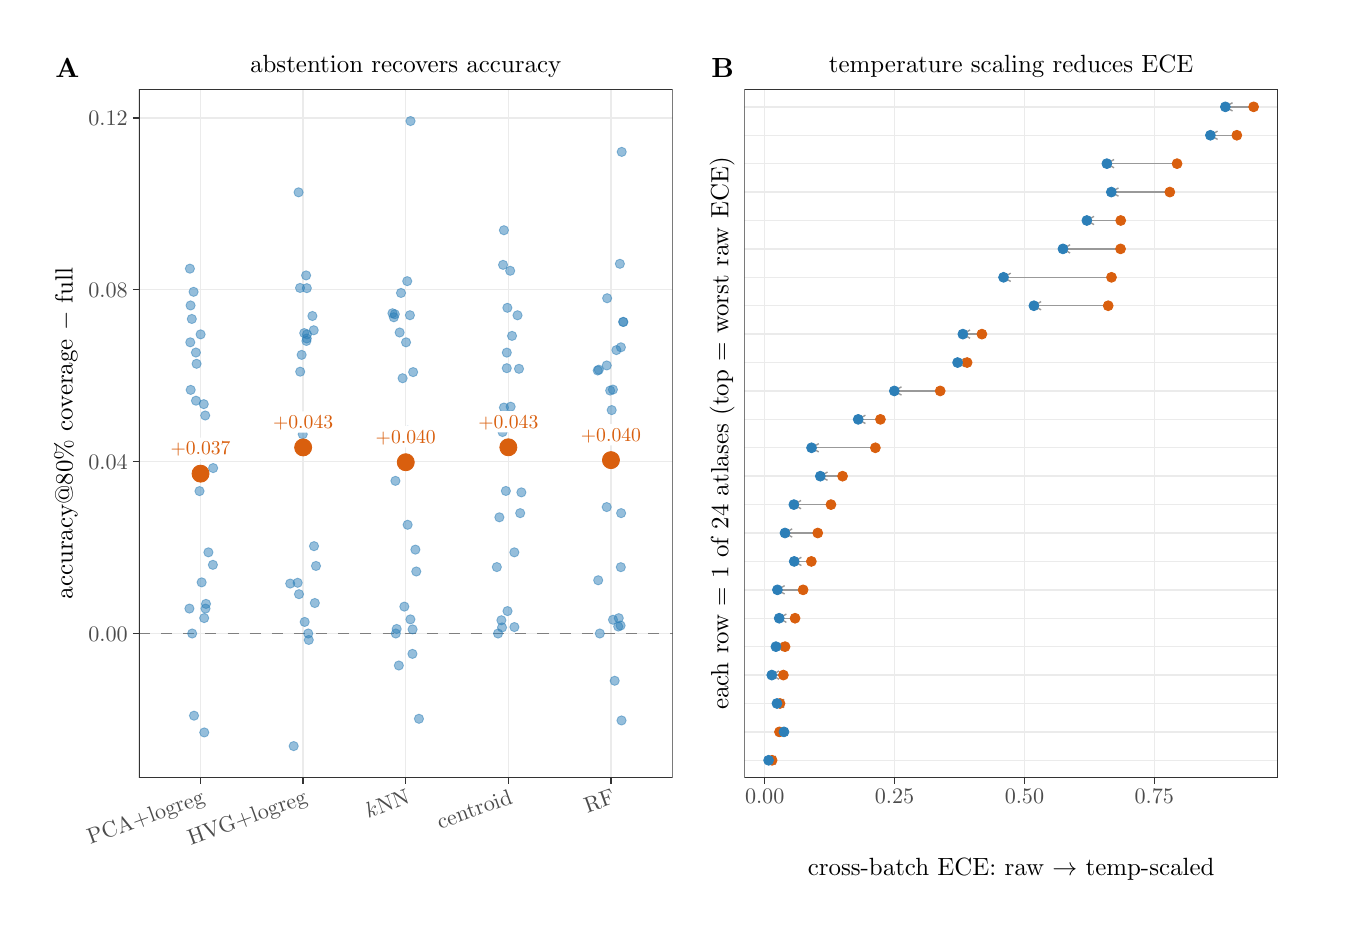
\begin{tikzpicture}[x=1pt,y=1pt]
\definecolor{fillColor}{RGB}{255,255,255}
\path[use as bounding box,fill=fillColor,fill opacity=0.00] (0,0) rectangle (469.75,317.99);
\begin{scope}
\path[clip] (  0.00,  0.00) rectangle (469.75,317.99);
\definecolor{drawColor}{RGB}{255,255,255}
\definecolor{fillColor}{RGB}{255,255,255}

\path[draw=drawColor,line width= 0.5pt,line join=round,line cap=round,fill=fillColor] (  0.00,  0.00) rectangle (469.75,317.99);
\end{scope}
\begin{scope}
\path[clip] (  5.00,  5.00) rectangle (242.01,312.99);
\definecolor{drawColor}{RGB}{255,255,255}
\definecolor{fillColor}{RGB}{255,255,255}

\path[draw=drawColor,line width= 0.5pt,line join=round,line cap=round,fill=fillColor] (  5.00,  5.00) rectangle (242.01,312.99);
\end{scope}
\begin{scope}
\path[clip] (242.01,  5.00) rectangle (460.75,312.99);
\definecolor{drawColor}{RGB}{255,255,255}
\definecolor{fillColor}{RGB}{255,255,255}

\path[draw=drawColor,line width= 0.5pt,line join=round,line cap=round,fill=fillColor] (242.01,  5.00) rectangle (460.76,312.99);
\end{scope}
\begin{scope}
\path[clip] ( 40.22, 47.10) rectangle (233.01,295.54);
\definecolor{fillColor}{RGB}{255,255,255}

\path[fill=fillColor] ( 40.22, 47.10) rectangle (233.01,295.54);
\definecolor{drawColor}{gray}{0.92}

\path[draw=drawColor,line width= 0.5pt,line join=round] ( 40.22, 99.07) --
	(233.01, 99.07);

\path[draw=drawColor,line width= 0.5pt,line join=round] ( 40.22,161.18) --
	(233.01,161.18);

\path[draw=drawColor,line width= 0.5pt,line join=round] ( 40.22,223.28) --
	(233.01,223.28);

\path[draw=drawColor,line width= 0.5pt,line join=round] ( 40.22,285.39) --
	(233.01,285.39);

\path[draw=drawColor,line width= 0.5pt,line join=round] ( 62.47, 47.10) --
	( 62.47,295.54);

\path[draw=drawColor,line width= 0.5pt,line join=round] ( 99.54, 47.10) --
	( 99.54,295.54);

\path[draw=drawColor,line width= 0.5pt,line join=round] (136.62, 47.10) --
	(136.62,295.54);

\path[draw=drawColor,line width= 0.5pt,line join=round] (173.69, 47.10) --
	(173.69,295.54);

\path[draw=drawColor,line width= 0.5pt,line join=round] (210.77, 47.10) --
	(210.77,295.54);
\definecolor{drawColor}{gray}{0.50}

\path[draw=drawColor,line width= 0.5pt,dash pattern=on 4pt off 4pt ,line join=round] ( 40.22, 99.07) -- (233.01, 99.07);
\definecolor{drawColor}{RGB}{44,127,184}
\definecolor{fillColor}{RGB}{44,127,184}

\path[draw=drawColor,draw opacity=0.50,line width= 0.3pt,line join=round,line cap=round,fill=fillColor,fill opacity=0.50] ( 63.81, 63.32) circle (  1.68);

\path[draw=drawColor,draw opacity=0.50,line width= 0.3pt,line join=round,line cap=round,fill=fillColor,fill opacity=0.50] (101.57, 96.74) circle (  1.68);

\path[draw=drawColor,draw opacity=0.50,line width= 0.3pt,line join=round,line cap=round,fill=fillColor,fill opacity=0.50] (133.34,100.71) circle (  1.68);

\path[draw=drawColor,draw opacity=0.50,line width= 0.3pt,line join=round,line cap=round,fill=fillColor,fill opacity=0.50] (171.18,103.86) circle (  1.68);

\path[draw=drawColor,draw opacity=0.50,line width= 0.3pt,line join=round,line cap=round,fill=fillColor,fill opacity=0.50] (211.51,104.04) circle (  1.68);

\path[draw=drawColor,draw opacity=0.50,line width= 0.3pt,line join=round,line cap=round,fill=fillColor,fill opacity=0.50] ( 66.93,123.88) circle (  1.68);

\path[draw=drawColor,draw opacity=0.50,line width= 0.3pt,line join=round,line cap=round,fill=fillColor,fill opacity=0.50] (104.18,123.48) circle (  1.68);

\path[draw=drawColor,draw opacity=0.50,line width= 0.3pt,line join=round,line cap=round,fill=fillColor,fill opacity=0.50] (140.42,121.48) circle (  1.68);

\path[draw=drawColor,draw opacity=0.50,line width= 0.3pt,line join=round,line cap=round,fill=fillColor,fill opacity=0.50] (169.53,123.08) circle (  1.68);

\path[draw=drawColor,draw opacity=0.50,line width= 0.3pt,line join=round,line cap=round,fill=fillColor,fill opacity=0.50] (206.16,118.31) circle (  1.68);

\path[draw=drawColor,draw opacity=0.50,line width= 0.3pt,line join=round,line cap=round,fill=fillColor,fill opacity=0.50] ( 62.09,150.53) circle (  1.68);

\path[draw=drawColor,draw opacity=0.50,line width= 0.3pt,line join=round,line cap=round,fill=fillColor,fill opacity=0.50] (103.47,130.64) circle (  1.68);

\path[draw=drawColor,draw opacity=0.50,line width= 0.3pt,line join=round,line cap=round,fill=fillColor,fill opacity=0.50] (137.34,172.33) circle (  1.68);

\path[draw=drawColor,draw opacity=0.50,line width= 0.3pt,line join=round,line cap=round,fill=fillColor,fill opacity=0.50] (174.35,230.14) circle (  1.68);

\path[draw=drawColor,draw opacity=0.50,line width= 0.3pt,line join=round,line cap=round,fill=fillColor,fill opacity=0.50] (209.23,144.76) circle (  1.68);

\path[draw=drawColor,draw opacity=0.50,line width= 0.3pt,line join=round,line cap=round,fill=fillColor,fill opacity=0.50] ( 65.31,128.40) circle (  1.68);

\path[draw=drawColor,draw opacity=0.50,line width= 0.3pt,line join=round,line cap=round,fill=fillColor,fill opacity=0.50] ( 97.55,117.40) circle (  1.68);

\path[draw=drawColor,draw opacity=0.50,line width= 0.3pt,line join=round,line cap=round,fill=fillColor,fill opacity=0.50] (137.29,138.36) circle (  1.68);

\path[draw=drawColor,draw opacity=0.50,line width= 0.3pt,line join=round,line cap=round,fill=fillColor,fill opacity=0.50] (177.97,142.56) circle (  1.68);

\path[draw=drawColor,draw opacity=0.50,line width= 0.3pt,line join=round,line cap=round,fill=fillColor,fill opacity=0.50] (214.44,142.57) circle (  1.68);

\path[draw=drawColor,draw opacity=0.50,line width= 0.3pt,line join=round,line cap=round,fill=fillColor,fill opacity=0.50] ( 67.02,158.85) circle (  1.68);

\path[draw=drawColor,draw opacity=0.50,line width= 0.3pt,line join=round,line cap=round,fill=fillColor,fill opacity=0.50] ( 99.71,175.04) circle (  1.68);

\path[draw=drawColor,draw opacity=0.50,line width= 0.3pt,line join=round,line cap=round,fill=fillColor,fill opacity=0.50] (134.41,207.84) circle (  1.68);

\path[draw=drawColor,draw opacity=0.50,line width= 0.3pt,line join=round,line cap=round,fill=fillColor,fill opacity=0.50] (172.09,244.79) circle (  1.68);

\path[draw=drawColor,draw opacity=0.50,line width= 0.3pt,line join=round,line cap=round,fill=fillColor,fill opacity=0.50] (212.74,201.48) circle (  1.68);

\path[draw=drawColor,draw opacity=0.50,line width= 0.3pt,line join=round,line cap=round,fill=fillColor,fill opacity=0.50] ( 63.78,104.64) circle (  1.68);

\path[draw=drawColor,draw opacity=0.50,line width= 0.3pt,line join=round,line cap=round,fill=fillColor,fill opacity=0.50] (100.09,103.25) circle (  1.68);

\path[draw=drawColor,draw opacity=0.50,line width= 0.3pt,line join=round,line cap=round,fill=fillColor,fill opacity=0.50] (138.30,104.18) circle (  1.68);

\path[draw=drawColor,draw opacity=0.50,line width= 0.3pt,line join=round,line cap=round,fill=fillColor,fill opacity=0.50] (175.88,101.40) circle (  1.68);

\path[draw=drawColor,draw opacity=0.50,line width= 0.3pt,line join=round,line cap=round,fill=fillColor,fill opacity=0.50] (214.25,101.95) circle (  1.68);

\path[draw=drawColor,draw opacity=0.50,line width= 0.3pt,line join=round,line cap=round,fill=fillColor,fill opacity=0.50] ( 58.86,217.61) circle (  1.68);

\path[draw=drawColor,draw opacity=0.50,line width= 0.3pt,line join=round,line cap=round,fill=fillColor,fill opacity=0.50] (102.89,213.80) circle (  1.68);

\path[draw=drawColor,draw opacity=0.50,line width= 0.3pt,line join=round,line cap=round,fill=fillColor,fill opacity=0.50] (135.48,191.31) circle (  1.68);

\path[draw=drawColor,draw opacity=0.50,line width= 0.3pt,line join=round,line cap=round,fill=fillColor,fill opacity=0.50] (171.78,232.28) circle (  1.68);

\path[draw=drawColor,draw opacity=0.50,line width= 0.3pt,line join=round,line cap=round,fill=fillColor,fill opacity=0.50] (209.39,220.22) circle (  1.68);

\path[draw=drawColor,draw opacity=0.50,line width= 0.3pt,line join=round,line cap=round,fill=fillColor,fill opacity=0.50] ( 64.43,109.77) circle (  1.68);

\path[draw=drawColor,draw opacity=0.50,line width= 0.3pt,line join=round,line cap=round,fill=fillColor,fill opacity=0.50] (103.76,110.09) circle (  1.68);

\path[draw=drawColor,draw opacity=0.50,line width= 0.3pt,line join=round,line cap=round,fill=fillColor,fill opacity=0.50] (136.11,108.79) circle (  1.68);

\path[draw=drawColor,draw opacity=0.50,line width= 0.3pt,line join=round,line cap=round,fill=fillColor,fill opacity=0.50] (173.39,107.17) circle (  1.68);

\path[draw=drawColor,draw opacity=0.50,line width= 0.3pt,line join=round,line cap=round,fill=fillColor,fill opacity=0.50] (213.58,104.62) circle (  1.68);

\path[draw=drawColor,draw opacity=0.50,line width= 0.3pt,line join=round,line cap=round,fill=fillColor,fill opacity=0.50] ( 61.03,196.53) circle (  1.68);

\path[draw=drawColor,draw opacity=0.50,line width= 0.3pt,line join=round,line cap=round,fill=fillColor,fill opacity=0.50] (100.87,223.86) circle (  1.68);

\path[draw=drawColor,draw opacity=0.50,line width= 0.3pt,line join=round,line cap=round,fill=fillColor,fill opacity=0.50] (132.89,154.23) circle (  1.68);

\path[draw=drawColor,draw opacity=0.50,line width= 0.3pt,line join=round,line cap=round,fill=fillColor,fill opacity=0.50] (178.40,150.07) circle (  1.68);

\path[draw=drawColor,draw opacity=0.50,line width= 0.3pt,line join=round,line cap=round,fill=fillColor,fill opacity=0.50] (210.48,186.86) circle (  1.68);

\path[draw=drawColor,draw opacity=0.50,line width= 0.3pt,line join=round,line cap=round,fill=fillColor,fill opacity=0.50] ( 63.63,181.95) circle (  1.68);

\path[draw=drawColor,draw opacity=0.50,line width= 0.3pt,line join=round,line cap=round,fill=fillColor,fill opacity=0.50] (103.36,208.65) circle (  1.68);

\path[draw=drawColor,draw opacity=0.50,line width= 0.3pt,line join=round,line cap=round,fill=fillColor,fill opacity=0.50] (136.72,204.28) circle (  1.68);

\path[draw=drawColor,draw opacity=0.50,line width= 0.3pt,line join=round,line cap=round,fill=fillColor,fill opacity=0.50] (172.09,180.72) circle (  1.68);

\path[draw=drawColor,draw opacity=0.50,line width= 0.3pt,line join=round,line cap=round,fill=fillColor,fill opacity=0.50] (214.37,202.49) circle (  1.68);

\path[draw=drawColor,draw opacity=0.50,line width= 0.3pt,line join=round,line cap=round,fill=fillColor,fill opacity=0.50] ( 59.31,212.73) circle (  1.68);

\path[draw=drawColor,draw opacity=0.50,line width= 0.3pt,line join=round,line cap=round,fill=fillColor,fill opacity=0.50] ( 98.42,223.94) circle (  1.68);

\path[draw=drawColor,draw opacity=0.50,line width= 0.3pt,line join=round,line cap=round,fill=fillColor,fill opacity=0.50] (137.15,226.39) circle (  1.68);

\path[draw=drawColor,draw opacity=0.50,line width= 0.3pt,line join=round,line cap=round,fill=fillColor,fill opacity=0.50] (173.12,194.94) circle (  1.68);

\path[draw=drawColor,draw opacity=0.50,line width= 0.3pt,line join=round,line cap=round,fill=fillColor,fill opacity=0.50] (213.99,232.66) circle (  1.68);

\path[draw=drawColor,draw opacity=0.50,line width= 0.3pt,line join=round,line cap=round,fill=fillColor,fill opacity=0.50] ( 59.95,222.54) circle (  1.68);

\path[draw=drawColor,draw opacity=0.50,line width= 0.3pt,line join=round,line cap=round,fill=fillColor,fill opacity=0.50] ( 98.99,199.75) circle (  1.68);

\path[draw=drawColor,draw opacity=0.50,line width= 0.3pt,line join=round,line cap=round,fill=fillColor,fill opacity=0.50] (132.66,214.45) circle (  1.68);

\path[draw=drawColor,draw opacity=0.50,line width= 0.3pt,line join=round,line cap=round,fill=fillColor,fill opacity=0.50] (171.41,175.60) circle (  1.68);

\path[draw=drawColor,draw opacity=0.50,line width= 0.3pt,line join=round,line cap=round,fill=fillColor,fill opacity=0.50] (205.98,194.11) circle (  1.68);

\path[draw=drawColor,draw opacity=0.50,line width= 0.3pt,line join=round,line cap=round,fill=fillColor,fill opacity=0.50] ( 59.44, 99.07) circle (  1.68);

\path[draw=drawColor,draw opacity=0.50,line width= 0.3pt,line join=round,line cap=round,fill=fillColor,fill opacity=0.50] (101.38, 99.07) circle (  1.68);

\path[draw=drawColor,draw opacity=0.50,line width= 0.3pt,line join=round,line cap=round,fill=fillColor,fill opacity=0.50] (133.02, 99.07) circle (  1.68);

\path[draw=drawColor,draw opacity=0.50,line width= 0.3pt,line join=round,line cap=round,fill=fillColor,fill opacity=0.50] (169.97, 99.07) circle (  1.68);

\path[draw=drawColor,draw opacity=0.50,line width= 0.3pt,line join=round,line cap=round,fill=fillColor,fill opacity=0.50] (206.74, 99.07) circle (  1.68);

\path[draw=drawColor,draw opacity=0.50,line width= 0.3pt,line join=round,line cap=round,fill=fillColor,fill opacity=0.50] ( 58.45,108.08) circle (  1.68);

\path[draw=drawColor,draw opacity=0.50,line width= 0.3pt,line join=round,line cap=round,fill=fillColor,fill opacity=0.50] ( 99.39,171.07) circle (  1.68);

\path[draw=drawColor,draw opacity=0.50,line width= 0.3pt,line join=round,line cap=round,fill=fillColor,fill opacity=0.50] (141.39, 68.26) circle (  1.68);

\path[draw=drawColor,draw opacity=0.50,line width= 0.3pt,line join=round,line cap=round,fill=fillColor,fill opacity=0.50] (172.80,150.58) circle (  1.68);

\path[draw=drawColor,draw opacity=0.50,line width= 0.3pt,line join=round,line cap=round,fill=fillColor,fill opacity=0.50] (214.33,123.04) circle (  1.68);

\path[draw=drawColor,draw opacity=0.50,line width= 0.3pt,line join=round,line cap=round,fill=fillColor,fill opacity=0.50] ( 62.49,207.16) circle (  1.68);

\path[draw=drawColor,draw opacity=0.50,line width= 0.3pt,line join=round,line cap=round,fill=fillColor,fill opacity=0.50] (100.86,205.67) circle (  1.68);

\path[draw=drawColor,draw opacity=0.50,line width= 0.3pt,line join=round,line cap=round,fill=fillColor,fill opacity=0.50] (132.30,213.34) circle (  1.68);

\path[draw=drawColor,draw opacity=0.50,line width= 0.3pt,line join=round,line cap=round,fill=fillColor,fill opacity=0.50] (173.34,216.76) circle (  1.68);

\path[draw=drawColor,draw opacity=0.50,line width= 0.3pt,line join=round,line cap=round,fill=fillColor,fill opacity=0.50] (206.37,194.39) circle (  1.68);

\path[draw=drawColor,draw opacity=0.50,line width= 0.3pt,line join=round,line cap=round,fill=fillColor,fill opacity=0.50] ( 64.16,177.85) circle (  1.68);

\path[draw=drawColor,draw opacity=0.50,line width= 0.3pt,line join=round,line cap=round,fill=fillColor,fill opacity=0.50] (100.61,228.46) circle (  1.68);

\path[draw=drawColor,draw opacity=0.50,line width= 0.3pt,line join=round,line cap=round,fill=fillColor,fill opacity=0.50] (138.13,214.08) circle (  1.68);

\path[draw=drawColor,draw opacity=0.50,line width= 0.3pt,line join=round,line cap=round,fill=fillColor,fill opacity=0.50] (175.02,206.61) circle (  1.68);

\path[draw=drawColor,draw opacity=0.50,line width= 0.3pt,line join=round,line cap=round,fill=fillColor,fill opacity=0.50] (211.48,187.22) circle (  1.68);

\path[draw=drawColor,draw opacity=0.50,line width= 0.3pt,line join=round,line cap=round,fill=fillColor,fill opacity=0.50] ( 60.11, 69.38) circle (  1.68);

\path[draw=drawColor,draw opacity=0.50,line width= 0.3pt,line join=round,line cap=round,fill=fillColor,fill opacity=0.50] ( 96.12, 58.39) circle (  1.68);

\path[draw=drawColor,draw opacity=0.50,line width= 0.3pt,line join=round,line cap=round,fill=fillColor,fill opacity=0.50] (134.12, 87.51) circle (  1.68);

\path[draw=drawColor,draw opacity=0.50,line width= 0.3pt,line join=round,line cap=round,fill=fillColor,fill opacity=0.50] (171.41,101.25) circle (  1.68);

\path[draw=drawColor,draw opacity=0.50,line width= 0.3pt,line join=round,line cap=round,fill=fillColor,fill opacity=0.50] (214.58, 67.65) circle (  1.68);

\path[draw=drawColor,draw opacity=0.50,line width= 0.3pt,line join=round,line cap=round,fill=fillColor,fill opacity=0.50] ( 60.82,183.20) circle (  1.68);

\path[draw=drawColor,draw opacity=0.50,line width= 0.3pt,line join=round,line cap=round,fill=fillColor,fill opacity=0.50] ( 99.93,207.63) circle (  1.68);

\path[draw=drawColor,draw opacity=0.50,line width= 0.3pt,line join=round,line cap=round,fill=fillColor,fill opacity=0.50] (140.10,129.38) circle (  1.68);

\path[draw=drawColor,draw opacity=0.50,line width= 0.3pt,line join=round,line cap=round,fill=fillColor,fill opacity=0.50] (174.52,181.03) circle (  1.68);

\path[draw=drawColor,draw opacity=0.50,line width= 0.3pt,line join=round,line cap=round,fill=fillColor,fill opacity=0.50] (211.03,179.80) circle (  1.68);

\path[draw=drawColor,draw opacity=0.50,line width= 0.3pt,line join=round,line cap=round,fill=fillColor,fill opacity=0.50] ( 58.76,204.29) circle (  1.68);

\path[draw=drawColor,draw opacity=0.50,line width= 0.3pt,line join=round,line cap=round,fill=fillColor,fill opacity=0.50] (100.94,207.16) circle (  1.68);

\path[draw=drawColor,draw opacity=0.50,line width= 0.3pt,line join=round,line cap=round,fill=fillColor,fill opacity=0.50] (134.90,222.13) circle (  1.68);

\path[draw=drawColor,draw opacity=0.50,line width= 0.3pt,line join=round,line cap=round,fill=fillColor,fill opacity=0.50] (177.00,214.06) circle (  1.68);

\path[draw=drawColor,draw opacity=0.50,line width= 0.3pt,line join=round,line cap=round,fill=fillColor,fill opacity=0.50] (209.25,195.93) circle (  1.68);

\path[draw=drawColor,draw opacity=0.50,line width= 0.3pt,line join=round,line cap=round,fill=fillColor,fill opacity=0.50] ( 64.25,108.07) circle (  1.68);

\path[draw=drawColor,draw opacity=0.50,line width= 0.3pt,line join=round,line cap=round,fill=fillColor,fill opacity=0.50] ( 98.04,113.28) circle (  1.68);

\path[draw=drawColor,draw opacity=0.50,line width= 0.3pt,line join=round,line cap=round,fill=fillColor,fill opacity=0.50] (139.04, 91.71) circle (  1.68);

\path[draw=drawColor,draw opacity=0.50,line width= 0.3pt,line join=round,line cap=round,fill=fillColor,fill opacity=0.50] (170.45,141.06) circle (  1.68);

\path[draw=drawColor,draw opacity=0.50,line width= 0.3pt,line join=round,line cap=round,fill=fillColor,fill opacity=0.50] (212.11, 81.99) circle (  1.68);

\path[draw=drawColor,draw opacity=0.50,line width= 0.3pt,line join=round,line cap=round,fill=fillColor,fill opacity=0.50] ( 58.90,187.10) circle (  1.68);

\path[draw=drawColor,draw opacity=0.50,line width= 0.3pt,line join=round,line cap=round,fill=fillColor,fill opacity=0.50] ( 98.48,193.68) circle (  1.68);

\path[draw=drawColor,draw opacity=0.50,line width= 0.3pt,line join=round,line cap=round,fill=fillColor,fill opacity=0.50] (131.81,214.79) circle (  1.68);

\path[draw=drawColor,draw opacity=0.50,line width= 0.3pt,line join=round,line cap=round,fill=fillColor,fill opacity=0.50] (173.13,200.57) circle (  1.68);

\path[draw=drawColor,draw opacity=0.50,line width= 0.3pt,line join=round,line cap=round,fill=fillColor,fill opacity=0.50] (215.16,211.67) circle (  1.68);

\path[draw=drawColor,draw opacity=0.50,line width= 0.3pt,line join=round,line cap=round,fill=fillColor,fill opacity=0.50] ( 60.79,200.60) circle (  1.68);

\path[draw=drawColor,draw opacity=0.50,line width= 0.3pt,line join=round,line cap=round,fill=fillColor,fill opacity=0.50] (100.73,204.78) circle (  1.68);

\path[draw=drawColor,draw opacity=0.50,line width= 0.3pt,line join=round,line cap=round,fill=fillColor,fill opacity=0.50] (139.28,193.53) circle (  1.68);

\path[draw=drawColor,draw opacity=0.50,line width= 0.3pt,line join=round,line cap=round,fill=fillColor,fill opacity=0.50] (171.60,171.88) circle (  1.68);

\path[draw=drawColor,draw opacity=0.50,line width= 0.3pt,line join=round,line cap=round,fill=fillColor,fill opacity=0.50] (215.27,211.65) circle (  1.68);

\path[draw=drawColor,draw opacity=0.50,line width= 0.3pt,line join=round,line cap=round,fill=fillColor,fill opacity=0.50] ( 58.62,230.91) circle (  1.68);

\path[draw=drawColor,draw opacity=0.50,line width= 0.3pt,line join=round,line cap=round,fill=fillColor,fill opacity=0.50] ( 97.89,258.49) circle (  1.68);

\path[draw=drawColor,draw opacity=0.50,line width= 0.3pt,line join=round,line cap=round,fill=fillColor,fill opacity=0.50] (138.34,284.25) circle (  1.68);

\path[draw=drawColor,draw opacity=0.50,line width= 0.3pt,line join=round,line cap=round,fill=fillColor,fill opacity=0.50] (177.54,194.72) circle (  1.68);

\path[draw=drawColor,draw opacity=0.50,line width= 0.3pt,line join=round,line cap=round,fill=fillColor,fill opacity=0.50] (214.65,273.10) circle (  1.68);

\path[draw=drawColor,draw opacity=0.50,line width= 0.3pt,line join=round,line cap=round,fill=fillColor,fill opacity=0.50] ( 62.86,117.55) circle (  1.68);

\path[draw=drawColor,draw opacity=0.50,line width= 0.3pt,line join=round,line cap=round,fill=fillColor,fill opacity=0.50] ( 94.87,117.12) circle (  1.68);

\path[draw=drawColor,draw opacity=0.50,line width= 0.3pt,line join=round,line cap=round,fill=fillColor,fill opacity=0.50] (139.08,100.56) circle (  1.68);

\path[draw=drawColor,draw opacity=0.50,line width= 0.3pt,line join=round,line cap=round,fill=fillColor,fill opacity=0.50] (175.86,128.40) circle (  1.68);

\path[draw=drawColor,draw opacity=0.50,line width= 0.3pt,line join=round,line cap=round,fill=fillColor,fill opacity=0.50] (213.40,101.59) circle (  1.68);
\definecolor{drawColor}{RGB}{217,95,14}
\definecolor{fillColor}{RGB}{217,95,14}

\path[draw=drawColor,line width= 0.3pt,line join=round,line cap=round,fill=fillColor] ( 62.47,156.83) circle (  3.08);

\path[draw=drawColor,line width= 0.3pt,line join=round,line cap=round,fill=fillColor] ( 99.54,166.31) circle (  3.08);

\path[draw=drawColor,line width= 0.3pt,line join=round,line cap=round,fill=fillColor] (136.62,160.96) circle (  3.08);

\path[draw=drawColor,line width= 0.3pt,line join=round,line cap=round,fill=fillColor] (173.69,166.36) circle (  3.08);

\path[draw=drawColor,line width= 0.3pt,line join=round,line cap=round,fill=fillColor] (210.77,161.72) circle (  3.08);
\definecolor{fillColor}{RGB}{255,255,255}

\path[fill=fillColor] ( 52.29,162.20) --
	( 72.65,162.20) --
	( 72.60,162.20) --
	( 72.80,162.21) --
	( 73.01,162.25) --
	( 73.20,162.33) --
	( 73.38,162.43) --
	( 73.54,162.56) --
	( 73.68,162.71) --
	( 73.79,162.89) --
	( 73.87,163.08) --
	( 73.92,163.28) --
	( 73.93,163.49) --
	( 73.93,163.49) --
	( 73.93,168.58) --
	( 73.93,168.58) --
	( 73.92,168.79) --
	( 73.87,168.99) --
	( 73.79,169.18) --
	( 73.68,169.35) --
	( 73.54,169.51) --
	( 73.38,169.64) --
	( 73.20,169.74) --
	( 73.01,169.82) --
	( 72.80,169.86) --
	( 72.65,169.87) --
	( 52.29,169.87) --
	( 52.44,169.86) --
	( 52.23,169.87) --
	( 52.03,169.84) --
	( 51.83,169.78) --
	( 51.64,169.69) --
	( 51.47,169.58) --
	( 51.32,169.43) --
	( 51.20,169.27) --
	( 51.10,169.09) --
	( 51.04,168.89) --
	( 51.00,168.69) --
	( 51.00,168.58) --
	( 51.00,163.49) --
	( 51.00,163.59) --
	( 51.00,163.38) --
	( 51.04,163.18) --
	( 51.10,162.98) --
	( 51.20,162.80) --
	( 51.32,162.63) --
	( 51.47,162.49) --
	( 51.64,162.37) --
	( 51.83,162.28) --
	( 52.03,162.23) --
	( 52.23,162.20) --
	cycle;
\end{scope}
\begin{scope}
\path[clip] ( 40.22, 47.10) rectangle (233.01,295.54);
\definecolor{drawColor}{RGB}{217,95,14}

\node[text=drawColor,anchor=base,inner sep=0pt, outer sep=0pt, scale=  0.71] at ( 62.47,163.58) {+0.037};
\end{scope}
\begin{scope}
\path[clip] ( 40.22, 47.10) rectangle (233.01,295.54);
\definecolor{fillColor}{RGB}{255,255,255}

\path[fill=fillColor] ( 89.36,171.68) --
	(109.72,171.68) --
	(109.67,171.68) --
	(109.88,171.69) --
	(110.08,171.73) --
	(110.28,171.80) --
	(110.45,171.90) --
	(110.61,172.04) --
	(110.75,172.19) --
	(110.86,172.36) --
	(110.94,172.56) --
	(110.99,172.76) --
	(111.01,172.96) --
	(111.01,172.96) --
	(111.01,178.06) --
	(111.01,178.06) --
	(110.99,178.26) --
	(110.94,178.46) --
	(110.86,178.66) --
	(110.75,178.83) --
	(110.61,178.98) --
	(110.45,179.12) --
	(110.28,179.22) --
	(110.08,179.29) --
	(109.88,179.33) --
	(109.72,179.34) --
	( 89.36,179.34) --
	( 89.52,179.33) --
	( 89.31,179.34) --
	( 89.10,179.32) --
	( 88.90,179.26) --
	( 88.72,179.17) --
	( 88.55,179.05) --
	( 88.40,178.91) --
	( 88.27,178.74) --
	( 88.18,178.56) --
	( 88.11,178.37) --
	( 88.08,178.16) --
	( 88.08,178.06) --
	( 88.08,172.96) --
	( 88.08,173.07) --
	( 88.08,172.86) --
	( 88.11,172.65) --
	( 88.18,172.46) --
	( 88.27,172.28) --
	( 88.40,172.11) --
	( 88.55,171.97) --
	( 88.72,171.85) --
	( 88.90,171.76) --
	( 89.10,171.70) --
	( 89.31,171.68) --
	cycle;
\end{scope}
\begin{scope}
\path[clip] ( 40.22, 47.10) rectangle (233.01,295.54);
\definecolor{drawColor}{RGB}{217,95,14}

\node[text=drawColor,anchor=base,inner sep=0pt, outer sep=0pt, scale=  0.71] at ( 99.54,173.06) {+0.043};
\end{scope}
\begin{scope}
\path[clip] ( 40.22, 47.10) rectangle (233.01,295.54);
\definecolor{fillColor}{RGB}{255,255,255}

\path[fill=fillColor] (126.44,166.32) --
	(146.80,166.32) --
	(146.75,166.32) --
	(146.95,166.33) --
	(147.16,166.37) --
	(147.35,166.45) --
	(147.53,166.55) --
	(147.69,166.68) --
	(147.83,166.84) --
	(147.94,167.01) --
	(148.02,167.20) --
	(148.07,167.40) --
	(148.09,167.61) --
	(148.09,167.61) --
	(148.09,172.70) --
	(148.09,172.70) --
	(148.07,172.91) --
	(148.02,173.11) --
	(147.94,173.30) --
	(147.83,173.48) --
	(147.69,173.63) --
	(147.53,173.76) --
	(147.35,173.87) --
	(147.16,173.94) --
	(146.95,173.98) --
	(146.80,173.99) --
	(126.44,173.99) --
	(126.59,173.98) --
	(126.38,173.99) --
	(126.18,173.96) --
	(125.98,173.91) --
	(125.79,173.82) --
	(125.62,173.70) --
	(125.47,173.56) --
	(125.35,173.39) --
	(125.25,173.21) --
	(125.19,173.01) --
	(125.15,172.81) --
	(125.15,172.70) --
	(125.15,167.61) --
	(125.15,167.71) --
	(125.15,167.51) --
	(125.19,167.30) --
	(125.25,167.10) --
	(125.35,166.92) --
	(125.47,166.76) --
	(125.62,166.61) --
	(125.79,166.50) --
	(125.98,166.41) --
	(126.18,166.35) --
	(126.38,166.32) --
	cycle;
\end{scope}
\begin{scope}
\path[clip] ( 40.22, 47.10) rectangle (233.01,295.54);
\definecolor{drawColor}{RGB}{217,95,14}

\node[text=drawColor,anchor=base,inner sep=0pt, outer sep=0pt, scale=  0.71] at (136.62,167.71) {+0.040};
\end{scope}
\begin{scope}
\path[clip] ( 40.22, 47.10) rectangle (233.01,295.54);
\definecolor{fillColor}{RGB}{255,255,255}

\path[fill=fillColor] (163.51,171.72) --
	(183.88,171.72) --
	(183.82,171.73) --
	(184.03,171.73) --
	(184.23,171.78) --
	(184.43,171.85) --
	(184.61,171.95) --
	(184.77,172.08) --
	(184.90,172.24) --
	(185.01,172.41) --
	(185.09,172.60) --
	(185.14,172.80) --
	(185.16,173.01) --
	(185.16,173.01) --
	(185.16,178.11) --
	(185.16,178.11) --
	(185.14,178.31) --
	(185.09,178.51) --
	(185.01,178.70) --
	(184.90,178.88) --
	(184.77,179.03) --
	(184.61,179.16) --
	(184.43,179.27) --
	(184.23,179.34) --
	(184.03,179.38) --
	(183.88,179.39) --
	(163.51,179.39) --
	(163.67,179.38) --
	(163.46,179.39) --
	(163.25,179.37) --
	(163.06,179.31) --
	(162.87,179.22) --
	(162.70,179.10) --
	(162.55,178.96) --
	(162.42,178.79) --
	(162.33,178.61) --
	(162.26,178.41) --
	(162.23,178.21) --
	(162.23,178.11) --
	(162.23,173.01) --
	(162.23,173.11) --
	(162.23,172.91) --
	(162.26,172.70) --
	(162.33,172.51) --
	(162.42,172.32) --
	(162.55,172.16) --
	(162.70,172.01) --
	(162.87,171.90) --
	(163.06,171.81) --
	(163.25,171.75) --
	(163.46,171.73) --
	cycle;
\end{scope}
\begin{scope}
\path[clip] ( 40.22, 47.10) rectangle (233.01,295.54);
\definecolor{drawColor}{RGB}{217,95,14}

\node[text=drawColor,anchor=base,inner sep=0pt, outer sep=0pt, scale=  0.71] at (173.69,173.11) {+0.043};
\end{scope}
\begin{scope}
\path[clip] ( 40.22, 47.10) rectangle (233.01,295.54);
\definecolor{fillColor}{RGB}{255,255,255}

\path[fill=fillColor] (200.59,167.08) --
	(220.95,167.08) --
	(220.90,167.08) --
	(221.11,167.09) --
	(221.31,167.13) --
	(221.50,167.21) --
	(221.68,167.31) --
	(221.84,167.44) --
	(221.98,167.60) --
	(222.09,167.77) --
	(222.17,167.96) --
	(222.22,168.16) --
	(222.24,168.37) --
	(222.24,168.37) --
	(222.24,173.46) --
	(222.24,173.46) --
	(222.22,173.67) --
	(222.17,173.87) --
	(222.09,174.06) --
	(221.98,174.24) --
	(221.84,174.39) --
	(221.68,174.52) --
	(221.50,174.62) --
	(221.31,174.70) --
	(221.11,174.74) --
	(220.95,174.75) --
	(200.59,174.75) --
	(200.74,174.74) --
	(200.53,174.75) --
	(200.33,174.72) --
	(200.13,174.66) --
	(199.94,174.58) --
	(199.77,174.46) --
	(199.62,174.32) --
	(199.50,174.15) --
	(199.40,173.97) --
	(199.34,173.77) --
	(199.31,173.57) --
	(199.30,173.46) --
	(199.30,168.37) --
	(199.31,168.47) --
	(199.31,168.26) --
	(199.34,168.06) --
	(199.40,167.86) --
	(199.50,167.68) --
	(199.62,167.52) --
	(199.77,167.37) --
	(199.94,167.25) --
	(200.13,167.17) --
	(200.33,167.11) --
	(200.53,167.08) --
	cycle;
\end{scope}
\begin{scope}
\path[clip] ( 40.22, 47.10) rectangle (233.01,295.54);
\definecolor{drawColor}{RGB}{217,95,14}

\node[text=drawColor,anchor=base,inner sep=0pt, outer sep=0pt, scale=  0.71] at (210.77,168.47) {+0.040};
\end{scope}
\begin{scope}
\path[clip] ( 40.22, 47.10) rectangle (233.01,295.54);
\definecolor{drawColor}{gray}{0.20}

\path[draw=drawColor,line width= 0.5pt,line join=round,line cap=round] ( 40.22, 47.10) rectangle (233.01,295.54);
\end{scope}
\begin{scope}
\path[clip] (  0.00,  0.00) rectangle (469.75,317.99);
\definecolor{drawColor}{gray}{0.30}

\node[text=drawColor,anchor=base east,inner sep=0pt, outer sep=0pt, scale=  0.80] at ( 36.17, 96.31) {0.00};

\node[text=drawColor,anchor=base east,inner sep=0pt, outer sep=0pt, scale=  0.80] at ( 36.17,158.42) {0.04};

\node[text=drawColor,anchor=base east,inner sep=0pt, outer sep=0pt, scale=  0.80] at ( 36.17,220.53) {0.08};

\node[text=drawColor,anchor=base east,inner sep=0pt, outer sep=0pt, scale=  0.80] at ( 36.17,282.64) {0.12};
\end{scope}
\begin{scope}
\path[clip] (  0.00,  0.00) rectangle (469.75,317.99);
\definecolor{drawColor}{gray}{0.20}

\path[draw=drawColor,line width= 0.5pt,line join=round] ( 37.97, 99.07) --
	( 40.22, 99.07);

\path[draw=drawColor,line width= 0.5pt,line join=round] ( 37.97,161.18) --
	( 40.22,161.18);

\path[draw=drawColor,line width= 0.5pt,line join=round] ( 37.97,223.28) --
	( 40.22,223.28);

\path[draw=drawColor,line width= 0.5pt,line join=round] ( 37.97,285.39) --
	( 40.22,285.39);
\end{scope}
\begin{scope}
\path[clip] (  0.00,  0.00) rectangle (469.75,317.99);
\definecolor{drawColor}{gray}{0.20}

\path[draw=drawColor,line width= 0.5pt,line join=round] ( 62.47, 44.85) --
	( 62.47, 47.10);

\path[draw=drawColor,line width= 0.5pt,line join=round] ( 99.54, 44.85) --
	( 99.54, 47.10);

\path[draw=drawColor,line width= 0.5pt,line join=round] (136.62, 44.85) --
	(136.62, 47.10);

\path[draw=drawColor,line width= 0.5pt,line join=round] (173.69, 44.85) --
	(173.69, 47.10);

\path[draw=drawColor,line width= 0.5pt,line join=round] (210.77, 44.85) --
	(210.77, 47.10);
\end{scope}
\begin{scope}
\path[clip] (  0.00,  0.00) rectangle (469.75,317.99);
\definecolor{drawColor}{gray}{0.30}

\node[text=drawColor,rotate= 20.00,anchor=base east,inner sep=0pt, outer sep=0pt, scale=  0.80] at ( 64.35, 37.87) {PCA+logreg};

\node[text=drawColor,rotate= 20.00,anchor=base east,inner sep=0pt, outer sep=0pt, scale=  0.80] at (101.43, 37.87) {HVG+logreg};

\node[text=drawColor,rotate= 20.00,anchor=base east,inner sep=0pt, outer sep=0pt, scale=  0.80] at (138.50, 37.87) {$k$NN};

\node[text=drawColor,rotate= 20.00,anchor=base east,inner sep=0pt, outer sep=0pt, scale=  0.80] at (175.58, 37.87) {centroid};

\node[text=drawColor,rotate= 20.00,anchor=base east,inner sep=0pt, outer sep=0pt, scale=  0.80] at (212.65, 37.87) {RF};
\end{scope}
\begin{scope}
\path[clip] (  0.00,  0.00) rectangle (469.75,317.99);
\definecolor{drawColor}{RGB}{0,0,0}

\node[text=drawColor,rotate= 90.00,anchor=base,inner sep=0pt, outer sep=0pt, scale=  0.90] at ( 16.20,171.32) {accuracy@80\% coverage $-$ full};
\end{scope}
\begin{scope}
\path[clip] (  0.00,  0.00) rectangle (469.75,317.99);
\definecolor{drawColor}{RGB}{0,0,0}

\node[text=drawColor,anchor=base,inner sep=0pt, outer sep=0pt, scale=  0.90] at (136.62,301.79) {abstention recovers accuracy};
\end{scope}
\begin{scope}
\path[clip] (  0.00,  0.00) rectangle (469.75,317.99);
\definecolor{drawColor}{RGB}{0,0,0}

\node[text=drawColor,anchor=base,inner sep=0pt, outer sep=0pt, scale=  1.00] at ( 14.35,300.03) {\bfseries A};
\end{scope}
\begin{scope}
\path[clip] (258.96, 47.10) rectangle (451.76,295.54);
\definecolor{fillColor}{RGB}{255,255,255}

\path[fill=fillColor] (258.96, 47.10) rectangle (451.75,295.54);
\definecolor{drawColor}{gray}{0.92}

\path[draw=drawColor,line width= 0.5pt,line join=round] (258.96, 53.26) --
	(451.76, 53.26);

\path[draw=drawColor,line width= 0.5pt,line join=round] (258.96, 63.52) --
	(451.76, 63.52);

\path[draw=drawColor,line width= 0.5pt,line join=round] (258.96, 73.79) --
	(451.76, 73.79);

\path[draw=drawColor,line width= 0.5pt,line join=round] (258.96, 84.05) --
	(451.76, 84.05);

\path[draw=drawColor,line width= 0.5pt,line join=round] (258.96, 94.32) --
	(451.76, 94.32);

\path[draw=drawColor,line width= 0.5pt,line join=round] (258.96,104.59) --
	(451.76,104.59);

\path[draw=drawColor,line width= 0.5pt,line join=round] (258.96,114.85) --
	(451.76,114.85);

\path[draw=drawColor,line width= 0.5pt,line join=round] (258.96,125.12) --
	(451.76,125.12);

\path[draw=drawColor,line width= 0.5pt,line join=round] (258.96,135.39) --
	(451.76,135.39);

\path[draw=drawColor,line width= 0.5pt,line join=round] (258.96,145.65) --
	(451.76,145.65);

\path[draw=drawColor,line width= 0.5pt,line join=round] (258.96,155.92) --
	(451.76,155.92);

\path[draw=drawColor,line width= 0.5pt,line join=round] (258.96,166.18) --
	(451.76,166.18);

\path[draw=drawColor,line width= 0.5pt,line join=round] (258.96,176.45) --
	(451.76,176.45);

\path[draw=drawColor,line width= 0.5pt,line join=round] (258.96,186.72) --
	(451.76,186.72);

\path[draw=drawColor,line width= 0.5pt,line join=round] (258.96,196.98) --
	(451.76,196.98);

\path[draw=drawColor,line width= 0.5pt,line join=round] (258.96,207.25) --
	(451.76,207.25);

\path[draw=drawColor,line width= 0.5pt,line join=round] (258.96,217.51) --
	(451.76,217.51);

\path[draw=drawColor,line width= 0.5pt,line join=round] (258.96,227.78) --
	(451.76,227.78);

\path[draw=drawColor,line width= 0.5pt,line join=round] (258.96,238.05) --
	(451.76,238.05);

\path[draw=drawColor,line width= 0.5pt,line join=round] (258.96,248.31) --
	(451.76,248.31);

\path[draw=drawColor,line width= 0.5pt,line join=round] (258.96,258.58) --
	(451.76,258.58);

\path[draw=drawColor,line width= 0.5pt,line join=round] (258.96,268.85) --
	(451.76,268.85);

\path[draw=drawColor,line width= 0.5pt,line join=round] (258.96,279.11) --
	(451.76,279.11);

\path[draw=drawColor,line width= 0.5pt,line join=round] (258.96,289.38) --
	(451.76,289.38);

\path[draw=drawColor,line width= 0.5pt,line join=round] (266.32, 47.10) --
	(266.32,295.54);

\path[draw=drawColor,line width= 0.5pt,line join=round] (313.25, 47.10) --
	(313.25,295.54);

\path[draw=drawColor,line width= 0.5pt,line join=round] (360.18, 47.10) --
	(360.18,295.54);

\path[draw=drawColor,line width= 0.5pt,line join=round] (407.11, 47.10) --
	(407.11,295.54);
\definecolor{drawColor}{gray}{0.60}

\path[draw=drawColor,line width= 0.5pt,line join=round] (436.93,279.11) -- (427.37,279.11);

\path[draw=drawColor,line width= 0.5pt,line join=round] (429.97,280.61) --
	(427.37,279.11) --
	(429.97,277.61);

\path[draw=drawColor,line width= 0.5pt,line join=round] (394.97,248.31) -- (382.73,248.31);

\path[draw=drawColor,line width= 0.5pt,line join=round] (385.33,249.81) --
	(382.73,248.31) --
	(385.33,246.81);

\path[draw=drawColor,line width= 0.5pt,line join=round] (329.74,186.72) -- (313.16,186.72);

\path[draw=drawColor,line width= 0.5pt,line join=round] (315.75,188.22) --
	(313.16,186.72) --
	(315.75,185.22);

\path[draw=drawColor,line width= 0.5pt,line join=round] (269.00, 53.26) -- (267.73, 53.26);

\path[draw=drawColor,line width= 0.5pt,line join=round] (270.32, 54.76) --
	(267.73, 53.26) --
	(270.32, 51.76);

\path[draw=drawColor,line width= 0.5pt,line join=round] (273.07, 84.05) -- (268.88, 84.05);

\path[draw=drawColor,line width= 0.5pt,line join=round] (271.47, 85.55) --
	(268.88, 84.05) --
	(271.47, 82.55);

\path[draw=drawColor,line width= 0.5pt,line join=round] (415.33,268.85) -- (389.96,268.85);

\path[draw=drawColor,line width= 0.5pt,line join=round] (392.56,270.35) --
	(389.96,268.85) --
	(392.56,267.35);

\path[draw=drawColor,line width= 0.5pt,line join=round] (339.47,196.98) -- (336.02,196.98);

\path[draw=drawColor,line width= 0.5pt,line join=round] (338.62,198.48) --
	(336.02,196.98) --
	(338.62,195.48);

\path[draw=drawColor,line width= 0.5pt,line join=round] (391.63,227.78) -- (352.63,227.78);

\path[draw=drawColor,line width= 0.5pt,line join=round] (355.22,229.28) --
	(352.63,227.78) --
	(355.22,226.28);

\path[draw=drawColor,line width= 0.5pt,line join=round] (273.68, 94.32) -- (270.38, 94.32);

\path[draw=drawColor,line width= 0.5pt,line join=round] (272.98, 95.82) --
	(270.38, 94.32) --
	(272.98, 92.82);

\path[draw=drawColor,line width= 0.5pt,line join=round] (294.46,155.92) -- (286.42,155.92);

\path[draw=drawColor,line width= 0.5pt,line join=round] (289.02,157.42) --
	(286.42,155.92) --
	(289.02,154.42);

\path[draw=drawColor,line width= 0.5pt,line join=round] (285.49,135.39) -- (273.65,135.39);

\path[draw=drawColor,line width= 0.5pt,line join=round] (276.25,136.89) --
	(273.65,135.39) --
	(276.25,133.89);

\path[draw=drawColor,line width= 0.5pt,line join=round] (308.14,176.45) -- (300.11,176.45);

\path[draw=drawColor,line width= 0.5pt,line join=round] (302.71,177.95) --
	(300.11,176.45) --
	(302.71,174.95);

\path[draw=drawColor,line width= 0.5pt,line join=round] (442.99,289.38) -- (432.78,289.38);

\path[draw=drawColor,line width= 0.5pt,line join=round] (435.37,290.88) --
	(432.78,289.38) --
	(435.37,287.88);

\path[draw=drawColor,line width= 0.5pt,line join=round] (344.81,207.25) -- (337.92,207.25);

\path[draw=drawColor,line width= 0.5pt,line join=round] (340.52,208.75) --
	(337.92,207.25) --
	(340.52,205.75);

\path[draw=drawColor,line width= 0.5pt,line join=round] (271.66, 63.52) -- (273.28, 63.52);

\path[draw=drawColor,line width= 0.5pt,line join=round] (270.68, 62.02) --
	(273.28, 63.52) --
	(270.68, 65.02);

\path[draw=drawColor,line width= 0.5pt,line join=round] (271.85, 73.79) -- (270.75, 73.79);

\path[draw=drawColor,line width= 0.5pt,line join=round] (273.35, 75.29) --
	(270.75, 73.79) --
	(273.35, 72.29);

\path[draw=drawColor,line width= 0.5pt,line join=round] (412.71,258.58) -- (391.57,258.58);

\path[draw=drawColor,line width= 0.5pt,line join=round] (394.16,260.08) --
	(391.57,258.58) --
	(394.16,257.08);

\path[draw=drawColor,line width= 0.5pt,line join=round] (283.18,125.12) -- (276.98,125.12);

\path[draw=drawColor,line width= 0.5pt,line join=round] (279.58,126.62) --
	(276.98,125.12) --
	(279.58,123.62);

\path[draw=drawColor,line width= 0.5pt,line join=round] (280.20,114.85) -- (270.92,114.85);

\path[draw=drawColor,line width= 0.5pt,line join=round] (273.52,116.35) --
	(270.92,114.85) --
	(273.52,113.35);

\path[draw=drawColor,line width= 0.5pt,line join=round] (390.44,217.51) -- (363.60,217.51);

\path[draw=drawColor,line width= 0.5pt,line join=round] (366.20,219.01) --
	(363.60,217.51) --
	(366.20,216.01);

\path[draw=drawColor,line width= 0.5pt,line join=round] (290.27,145.65) -- (276.86,145.65);

\path[draw=drawColor,line width= 0.5pt,line join=round] (279.46,147.15) --
	(276.86,145.65) --
	(279.46,144.15);

\path[draw=drawColor,line width= 0.5pt,line join=round] (306.32,166.18) -- (283.25,166.18);

\path[draw=drawColor,line width= 0.5pt,line join=round] (285.85,167.68) --
	(283.25,166.18) --
	(285.85,164.68);

\path[draw=drawColor,line width= 0.5pt,line join=round] (277.29,104.59) -- (271.56,104.59);

\path[draw=drawColor,line width= 0.5pt,line join=round] (274.15,106.09) --
	(271.56,104.59) --
	(274.15,103.09);

\path[draw=drawColor,line width= 0.5pt,line join=round] (394.91,238.05) -- (374.09,238.05);

\path[draw=drawColor,line width= 0.5pt,line join=round] (376.68,239.55) --
	(374.09,238.05) --
	(376.68,236.55);
\definecolor{drawColor}{RGB}{217,95,14}
\definecolor{fillColor}{RGB}{217,95,14}

\path[draw=drawColor,line width= 0.3pt,line join=round,line cap=round,fill=fillColor] (436.93,279.11) circle (  1.79);

\path[draw=drawColor,line width= 0.3pt,line join=round,line cap=round,fill=fillColor] (394.97,248.31) circle (  1.79);

\path[draw=drawColor,line width= 0.3pt,line join=round,line cap=round,fill=fillColor] (329.74,186.72) circle (  1.79);

\path[draw=drawColor,line width= 0.3pt,line join=round,line cap=round,fill=fillColor] (269.00, 53.26) circle (  1.79);

\path[draw=drawColor,line width= 0.3pt,line join=round,line cap=round,fill=fillColor] (273.07, 84.05) circle (  1.79);

\path[draw=drawColor,line width= 0.3pt,line join=round,line cap=round,fill=fillColor] (415.33,268.85) circle (  1.79);

\path[draw=drawColor,line width= 0.3pt,line join=round,line cap=round,fill=fillColor] (339.47,196.98) circle (  1.79);

\path[draw=drawColor,line width= 0.3pt,line join=round,line cap=round,fill=fillColor] (391.63,227.78) circle (  1.79);

\path[draw=drawColor,line width= 0.3pt,line join=round,line cap=round,fill=fillColor] (273.68, 94.32) circle (  1.79);

\path[draw=drawColor,line width= 0.3pt,line join=round,line cap=round,fill=fillColor] (294.46,155.92) circle (  1.79);

\path[draw=drawColor,line width= 0.3pt,line join=round,line cap=round,fill=fillColor] (285.49,135.39) circle (  1.79);

\path[draw=drawColor,line width= 0.3pt,line join=round,line cap=round,fill=fillColor] (308.14,176.45) circle (  1.79);

\path[draw=drawColor,line width= 0.3pt,line join=round,line cap=round,fill=fillColor] (442.99,289.38) circle (  1.79);

\path[draw=drawColor,line width= 0.3pt,line join=round,line cap=round,fill=fillColor] (344.81,207.25) circle (  1.79);

\path[draw=drawColor,line width= 0.3pt,line join=round,line cap=round,fill=fillColor] (271.66, 63.52) circle (  1.79);

\path[draw=drawColor,line width= 0.3pt,line join=round,line cap=round,fill=fillColor] (271.85, 73.79) circle (  1.79);

\path[draw=drawColor,line width= 0.3pt,line join=round,line cap=round,fill=fillColor] (412.71,258.58) circle (  1.79);

\path[draw=drawColor,line width= 0.3pt,line join=round,line cap=round,fill=fillColor] (283.18,125.12) circle (  1.79);

\path[draw=drawColor,line width= 0.3pt,line join=round,line cap=round,fill=fillColor] (280.20,114.85) circle (  1.79);

\path[draw=drawColor,line width= 0.3pt,line join=round,line cap=round,fill=fillColor] (390.44,217.51) circle (  1.79);

\path[draw=drawColor,line width= 0.3pt,line join=round,line cap=round,fill=fillColor] (290.27,145.65) circle (  1.79);

\path[draw=drawColor,line width= 0.3pt,line join=round,line cap=round,fill=fillColor] (306.32,166.18) circle (  1.79);

\path[draw=drawColor,line width= 0.3pt,line join=round,line cap=round,fill=fillColor] (277.29,104.59) circle (  1.79);

\path[draw=drawColor,line width= 0.3pt,line join=round,line cap=round,fill=fillColor] (394.91,238.05) circle (  1.79);
\definecolor{drawColor}{RGB}{44,127,184}
\definecolor{fillColor}{RGB}{44,127,184}

\path[draw=drawColor,line width= 0.3pt,line join=round,line cap=round,fill=fillColor] (427.37,279.11) circle (  1.79);

\path[draw=drawColor,line width= 0.3pt,line join=round,line cap=round,fill=fillColor] (382.73,248.31) circle (  1.79);

\path[draw=drawColor,line width= 0.3pt,line join=round,line cap=round,fill=fillColor] (313.16,186.72) circle (  1.79);

\path[draw=drawColor,line width= 0.3pt,line join=round,line cap=round,fill=fillColor] (267.73, 53.26) circle (  1.79);

\path[draw=drawColor,line width= 0.3pt,line join=round,line cap=round,fill=fillColor] (268.88, 84.05) circle (  1.79);

\path[draw=drawColor,line width= 0.3pt,line join=round,line cap=round,fill=fillColor] (389.96,268.85) circle (  1.79);

\path[draw=drawColor,line width= 0.3pt,line join=round,line cap=round,fill=fillColor] (336.02,196.98) circle (  1.79);

\path[draw=drawColor,line width= 0.3pt,line join=round,line cap=round,fill=fillColor] (352.63,227.78) circle (  1.79);

\path[draw=drawColor,line width= 0.3pt,line join=round,line cap=round,fill=fillColor] (270.38, 94.32) circle (  1.79);

\path[draw=drawColor,line width= 0.3pt,line join=round,line cap=round,fill=fillColor] (286.42,155.92) circle (  1.79);

\path[draw=drawColor,line width= 0.3pt,line join=round,line cap=round,fill=fillColor] (273.65,135.39) circle (  1.79);

\path[draw=drawColor,line width= 0.3pt,line join=round,line cap=round,fill=fillColor] (300.11,176.45) circle (  1.79);

\path[draw=drawColor,line width= 0.3pt,line join=round,line cap=round,fill=fillColor] (432.78,289.38) circle (  1.79);

\path[draw=drawColor,line width= 0.3pt,line join=round,line cap=round,fill=fillColor] (337.92,207.25) circle (  1.79);

\path[draw=drawColor,line width= 0.3pt,line join=round,line cap=round,fill=fillColor] (273.28, 63.52) circle (  1.79);

\path[draw=drawColor,line width= 0.3pt,line join=round,line cap=round,fill=fillColor] (270.75, 73.79) circle (  1.79);

\path[draw=drawColor,line width= 0.3pt,line join=round,line cap=round,fill=fillColor] (391.57,258.58) circle (  1.79);

\path[draw=drawColor,line width= 0.3pt,line join=round,line cap=round,fill=fillColor] (276.98,125.12) circle (  1.79);

\path[draw=drawColor,line width= 0.3pt,line join=round,line cap=round,fill=fillColor] (270.92,114.85) circle (  1.79);

\path[draw=drawColor,line width= 0.3pt,line join=round,line cap=round,fill=fillColor] (363.60,217.51) circle (  1.79);

\path[draw=drawColor,line width= 0.3pt,line join=round,line cap=round,fill=fillColor] (276.86,145.65) circle (  1.79);

\path[draw=drawColor,line width= 0.3pt,line join=round,line cap=round,fill=fillColor] (283.25,166.18) circle (  1.79);

\path[draw=drawColor,line width= 0.3pt,line join=round,line cap=round,fill=fillColor] (271.56,104.59) circle (  1.79);

\path[draw=drawColor,line width= 0.3pt,line join=round,line cap=round,fill=fillColor] (374.09,238.05) circle (  1.79);
\definecolor{drawColor}{gray}{0.20}

\path[draw=drawColor,line width= 0.5pt,line join=round,line cap=round] (258.96, 47.10) rectangle (451.75,295.54);
\end{scope}
\begin{scope}
\path[clip] (  0.00,  0.00) rectangle (469.75,317.99);
\definecolor{drawColor}{gray}{0.20}

\path[draw=drawColor,line width= 0.5pt,line join=round] (266.32, 44.85) --
	(266.32, 47.10);

\path[draw=drawColor,line width= 0.5pt,line join=round] (313.25, 44.85) --
	(313.25, 47.10);

\path[draw=drawColor,line width= 0.5pt,line join=round] (360.18, 44.85) --
	(360.18, 47.10);

\path[draw=drawColor,line width= 0.5pt,line join=round] (407.11, 44.85) --
	(407.11, 47.10);
\end{scope}
\begin{scope}
\path[clip] (  0.00,  0.00) rectangle (469.75,317.99);
\definecolor{drawColor}{gray}{0.30}

\node[text=drawColor,anchor=base,inner sep=0pt, outer sep=0pt, scale=  0.80] at (266.32, 37.53) {0.00};

\node[text=drawColor,anchor=base,inner sep=0pt, outer sep=0pt, scale=  0.80] at (313.25, 37.53) {0.25};

\node[text=drawColor,anchor=base,inner sep=0pt, outer sep=0pt, scale=  0.80] at (360.18, 37.53) {0.50};

\node[text=drawColor,anchor=base,inner sep=0pt, outer sep=0pt, scale=  0.80] at (407.11, 37.53) {0.75};
\end{scope}
\begin{scope}
\path[clip] (  0.00,  0.00) rectangle (469.75,317.99);
\definecolor{drawColor}{RGB}{0,0,0}

\node[text=drawColor,anchor=base,inner sep=0pt, outer sep=0pt, scale=  0.90] at (355.36, 11.75) {cross-batch ECE: raw $\to$ temp-scaled};
\end{scope}
\begin{scope}
\path[clip] (  0.00,  0.00) rectangle (469.75,317.99);
\definecolor{drawColor}{RGB}{0,0,0}

\node[text=drawColor,rotate= 90.00,anchor=base,inner sep=0pt, outer sep=0pt, scale=  0.90] at (253.21,171.32) {each row $=$ 1 of 24 atlases (top $=$ worst raw ECE)};
\end{scope}
\begin{scope}
\path[clip] (  0.00,  0.00) rectangle (469.75,317.99);
\definecolor{drawColor}{RGB}{0,0,0}

\node[text=drawColor,anchor=base,inner sep=0pt, outer sep=0pt, scale=  0.90] at (355.36,301.79) {temperature scaling reduces ECE};
\end{scope}
\begin{scope}
\path[clip] (  0.00,  0.00) rectangle (469.75,317.99);
\definecolor{drawColor}{RGB}{0,0,0}

\node[text=drawColor,anchor=base,inner sep=0pt, outer sep=0pt, scale=  1.00] at (251.10,300.03) {\bfseries B};
\end{scope}
\end{tikzpicture}
